\section{Introduction}\label{sec:intro}

Middleboxes such as firewalls, NATs, and proxies, have grown to be a vital part of modern networks but are 
also widely recognized as bringing  with them significant problems including high cost, inflexibility, and complex management.  
These problems have led both research and industry to explore an alternate approach: moving middlebox functionality out of dedicated boxes and into 
software applications that run multiplexed on commodity server hardware~\cite{mb-manifesto,comb,aplomb,opennf,clickos,flowtags,nfv,domain20,opnfv}.
This approach -- termed Network Function Virtualization (NFV) in industry -- promises many advantages including: the cost benefits of commodity infrastructure, 
the efficiencies of statistical multiplexing, and the flexibility of software solutions. 
In a short time, NFV has significant momentum with over 270 industry participants~\cite{etsi-nfv} and a number of emerging product offerings~\cite{something}.

Leveraging the above trend, several efforts are exploring a new model for middlebox deployment in which a third-party offers middlebox processing as a  
\emph{service}.
Such a middlebox service may be hosted in a public cloud~\cite{aplomb,zscalar,aryaka} or in private clouds embedded within ISP 
infrastructure~\cite{domain20, telefonica}.  
This service model allows customers such as enterprises to ``outsource'' middleboxes from their networks entirely, and hence promises many of the same 
benefits that outsourcing compute and storage have attained through cloud computing.%: decreased costs, ease of management, \etc{}.

However, outsourcing middleboxes to a third party provider brings a new challenge: the confidentiality of the traffic. 
Today, in order to process an organization's traffic, the cloud receives the traffic {\em unencrypted}.  This means that the cloud 
now has access to potentially sensitive packet payloads,  IP addresses, and ports. This is 
worrisome considering the number of documented data breaches by cloud employees or hackers~\cite{PrivacyRecords}.
Hence, an important question is: can we enable a third party to perform traffic processing for an enterprise, {\em without seeing the enterprise's traffic}?
   
In recent work, we addressed this challenge for one type of middlebox: Intrusion Detection Systems (IDS)~\cite{blindbox}.  
We developed BlindBox, a system that uses new encryption schemes to enable IDS processing directly on \emph{encrypted} traffic.\footnote{Say something 
about other SIGCOMM paper.}
In BlindBox, traffic is encrypted at the user and the cloud processes this encrypted traffic without ever decrypting it. 
%Since the service provider receives only encrypted traffic and no decryption key, it cannot see the confidential data. 
BlindBox offers a valuable first step towards simultaneously achieving both the functionality of middleboxes and the privacy of encryption. 
However, it suffers from two non-trivial limitations.% that make it impractical for deployment today. 

First, BlindBox's approach does not generalize to middleboxes beyond IDS but a compelling middlebox service must support a wide range of middleboxes such as 
NAT, firewalls, proxies, and load balancers. Moreover, even in the context of IDS, BlindBox only supports exact-match operations on encrypted traffic. 
For more complex rules (e.g., rules with regular expressions or scripts), BlindBox requires that operators identify a `pre-filter' based on 
exact-match operations; if a packet matches the pre-filter, it is decrypted for further processing. For real-world rulesets, BlindBox thus resorts
 to decrypting traffic for between 33-77\% of rules~\cite{blindbox}. 

The second limitation is that components of BlindBox introduce performance overheads that are so high as to make deployment impractical. 
Specifically, connection setup times in BlindBox are proportional to the number of IDS rules and can take as much as 97 seconds per connection 
for rulesets with thousands of attack rules. 

In this paper, we present \sys,\footnote{\sys's name concatenates the words MB (middlebox) and Ark (protection).}
 a system that combines novel cryptographic and systems techniques to resolve the above limitations for 
 the context in which users reside in a trusted network environment such as an enterprise or campus. 
This context is an important one as it represents the majority of middlebox usage today~\cite{need-citation}. 

\sys is the first system that enables running a wide range of middleboxes as a cloud service while maintaining confidentiality of the traffic, 
and to do so with practical performance. 
\sys provides these guarantees even against attackers who gain access to {\em all} the data at the cloud. 
\sys supports all middleboxes that \cite{aplomb} documents to be fit for cloud outsourcing.   
In addition, for IDS, \sys can avoid decrypting traffic for between {\bf X-Y\%} of rules (an almost {\bf Z\%} improvement over \cite{blindbox}). 
\sys achieves the above with very low performance overhead, degrading throughput by only {\bf P\%} compared to systems that 
process unencrypted traffic~\cite{aplomb}. \sr{latency?}
\sys is designed for enterprise or campus users and is not appropriate for users that access the network from untrusted or unmanaged environments 
such as the home or public cafes \sr{fix}. 

In what follows, we explain the key insights that drive \sys's design (\S\ref{sec:approach}) and then summarize our contributions (\S\ref{sec:contributions}). 


%Like BlindBox, the approach in \sys is to encrypt the traffic that goes to the middleboxes in the cloud and enable the cloud to process encrypted traffic without ever decrypting it. 
%\sys encrypts the packet payload as well as important information in the header (such as IP addresses and ports). 

\subsection{Approach} 
\label{sec:approach}
\sys is built on two insights that allow us to overcome the limitations of BlindBox.  

First, we observe that two core operations underlie a range of middlebox processing: {\em keyword match} and {\em range match}. Keyword match refers to identifying if 
a keyword appears in a byte stream. For example, a web proxy uses keyword match to identify if a cached filename appears in a HTTP GET request. 
Range match enables determining if a value $x$ lies in an interval [$x_1$, $x_2$]; e.g., if an IP address lies in [18.0.0.0, 18.255.255.255] (\ie{} the 
prefix 18.0.0.0/8). 

Although there exist algorithms for keyword match, there is no suitable encryption scheme for range match operations.  
As we elaborate on in \S\ref{sec:buildingblocks}, the only practical schemes applicable here perform order-preserving encryption (OPE)~\cite{boldyreva:ope,popa:mope}, and 
are both too insecure and too slow for our setting. For example, OPE schemes leak the order of the values encrypted. 

We thus designed a new encryption scheme, called {\em RangeMatch}, which is targeted at and takes advantage of the network setting. 
RangeMatch is fast (performing encryptions in under 3$\mu$s which, 3 orders of magnitude faster than OPE schemes) and it is more secure because 
it does not reveal the order of the values encrypted. 
By appropriately combining RangeMatch with BlindBox's solution for keyword matching, \sys is able to support a wide range of middleboxes, thereby 
achieving generality. Table~\ref{tab:apps-ops} summarizes the middleboxes we support and the operations they rely on. 

Our second insight derives from the system context we focus on: 
that in which an administrative domain such as an enterprise chooses to outsource their middlebox processing to a third-party service. 
In this context, the enterprise acts as an intermediary on the data path between the end-user and the middlebox provider; 
specifically, packets flowing to/from the enterprise user will naturally traverse some form of \emph{gateway} in the enterprise network. 
We design \sys to exploit the presence of this gateway to both eliminate the performance limitations of BlindBox as well as 
expand BlindBox's coverage of IDS.

In \sys, the expensive setup that BlindBox requires is only done once (between the gateway and the middlebox provider) rather 
than afresh for each new connection. This eliminates the performance bottleneck that renders BlindBox impractical. 
Moreover, because performance is no longer proportional to the number of rules, we can expand BlindBox's ability to deal with   
rules that include regular expressions by simply expanding such expressions into distinct rules. This simple approach allows us 
 to increase the number of rules that can be processed without decryption by {\bf X-Y\%}. Thus, not only is \sys more 
general (i.e., supporting middleboxes beyond IDS), it also greatly improves on the state-of-the-art for IDS processing in terms 
of both performance and security. 

Finally, \sys also exploits the existence of the enterprise gateway to improve deployability by (re)factoring functionality to shift 
operations away from the end-user and into the gateway. This results in a design that, in contrast to BlindBox, requires: (i) no 
change at end users and (ii) no change to middlebox `fast path' algorithms (e.g., for packet classification or IP lookups~\cite{varghese, mckeown, long, list}) 
that have been honed over decades to meet line speeds. 


\subsection{Contributions}
\label{sec:contributions}

In this paper, we make the following contributions: 

\begin{itemize} 
\item We present RangeMatch, a new encryption scheme that supports range-match operations directly on encrypted data. RangeMatch is 
3 orders of magnitude faster and more secure than existing OPE approaches
\item For keyword matching as required by IDS, we adopt the solutions of BlindBox and show how to improve them. For the context of enterprise 
users, we reduce BlindBox's performance overheads by {\bf X\%} and almost double the number of IDS rules that BlindBox can process without resorting 
to decryption. 
\item We show how to integrate RangeMatch and keyword matching to support processing encrypted traffic for the 
range of middleboxes shown in Table~\ref{tab:apps-ops}. 
\item We design and implement a practical system for middlebox processing on encrypted traffic. Our system, \sys,   
can be deployed with no change at end users and no change to middlebox fast-path algorithms. 
\vspace{-0.4em}
\item We deploy \sys on EC2 and show that our design suffers a throughput penalty of only {\bf X\%} relative to processing unencrypted 
traffic~\cite{aplomb}.  
\vspace{-0.4em}
\end{itemize} 

The remainder of this paper is organized as follows: \ldots. 
 


    
\newcounter{theapp} \setcounter{theapp}{0}  
\newcommand{\capp}{\refstepcounter{theapp}\arabic{theapp}}
    
\begin{table}[t!]
\centering  
\begin{tabular}{c|p{3.6cm}|p{0.6cm}|p{2.25cm}}
& {\bf Middlebox}  & {\bf Type } & {\bf Example}  \\
\hline \hline
\capp &  IP Firewall \S\ref{sec:firewall} & HO &  IP address   \\
\capp &  Application Firewall  \S\ref{sec:firewall} & BA & IP address  \\
\capp & NAT  \S\ref{sec:nat} & HO & IP address  \\
\capp & IP Forwarding  \S\ref{sec:other_apps}  & HO &  IP address \\
\capp & Load Balancer L4 \S\ref{sec:loadb} & HO & IP address  \\
\capp & Load Balancer L7 \S\ref{sec:loadb} & BA & URL in payload  \\
\capp & Web Proxy/Cache  \S\ref{s:proxy} & HO & URL in payload \\
\capp & Intrusion Detect (IDS) \S\ref{sec:ids} & BA & payload \\
\capp & Data Exfiltration  \S\ref{sec:ids} & BA & payload \\
\capp & VPN Gateway \S\ref{sec:vpn} &  HO &  IP address \\ 
\end{tabular}
\caption{Middleboxes supported by \sys, shown with the section that discusses them, their type, HO (header only) or BA (bytestream aware), and one  example of an encrypted field  each operates on. \label{tab:apps-ops} }
\end{table}

% 2nd fig/1st fig = 1.12 ratio
\begin{figure*}[t!]
\centering
\hspace{.2in}
\subfigure[Enterprise to external site communication]{
  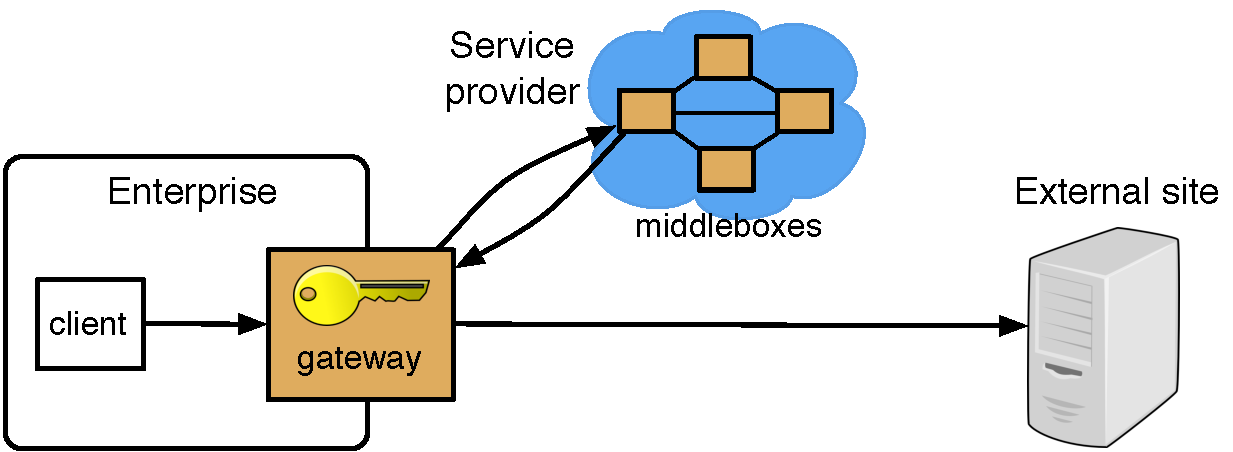
\includegraphics[width=2.5in]{fig/model_1.pdf}
  \label{fig:model1} }
%
\subfigure[Enterprise to enterprise communication]{
   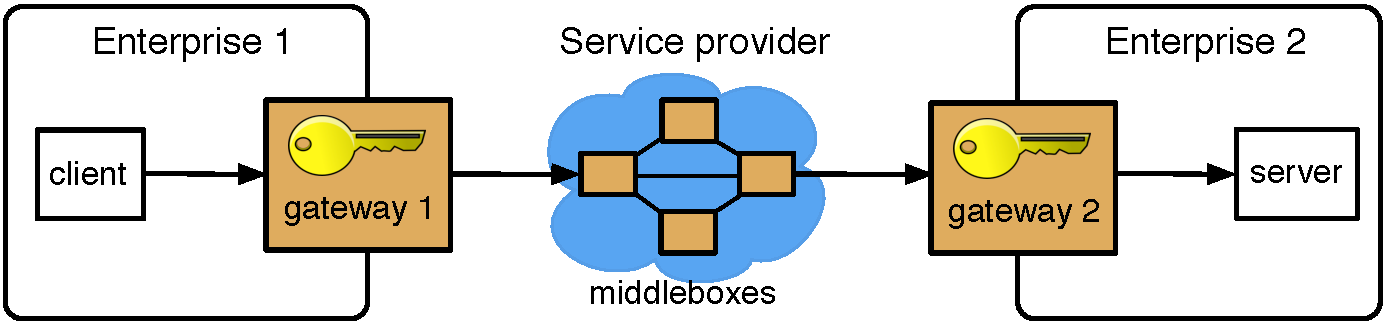
\includegraphics[width=3.0in]{fig/model_2.pdf}
     \label{fig:model2}}
     %
\caption{System architecture. Aplomb and NFV system setup with \sys encryption  at the gateway. The arrows indicate traffic from the client to the server; the response traffic follows the reverse direction. \label{fig:sys-overview}}
\end{figure*}


\eat{ 
 data plane which processes packets. In particular, firewalls implemented in hardware can use the existing hardware unchanged.  This enables middlebox throughput with \sys to almost match throughput without \sys, despite our changes.

We implemented and evaluated \sys on EC2. 
Further, \sys imposes negligible throughput overheads at the service provider: for example, a firewall operating over encrypted data achieves 9.8Gbps, equal to the same firewall over unencrypted data.
Our gateway can forward at 1.5 Gbps on a single core; our 8 core server can transmit \sys encrypted data at up to 8Gbps.% line rate of its network interface.
}
